\documentclass[12pt, aspectration=54, UTF8]{beamer}
\usetheme{Boadilla}
\usefonttheme{serif} 
\setbeamertemplate{background} 
{
    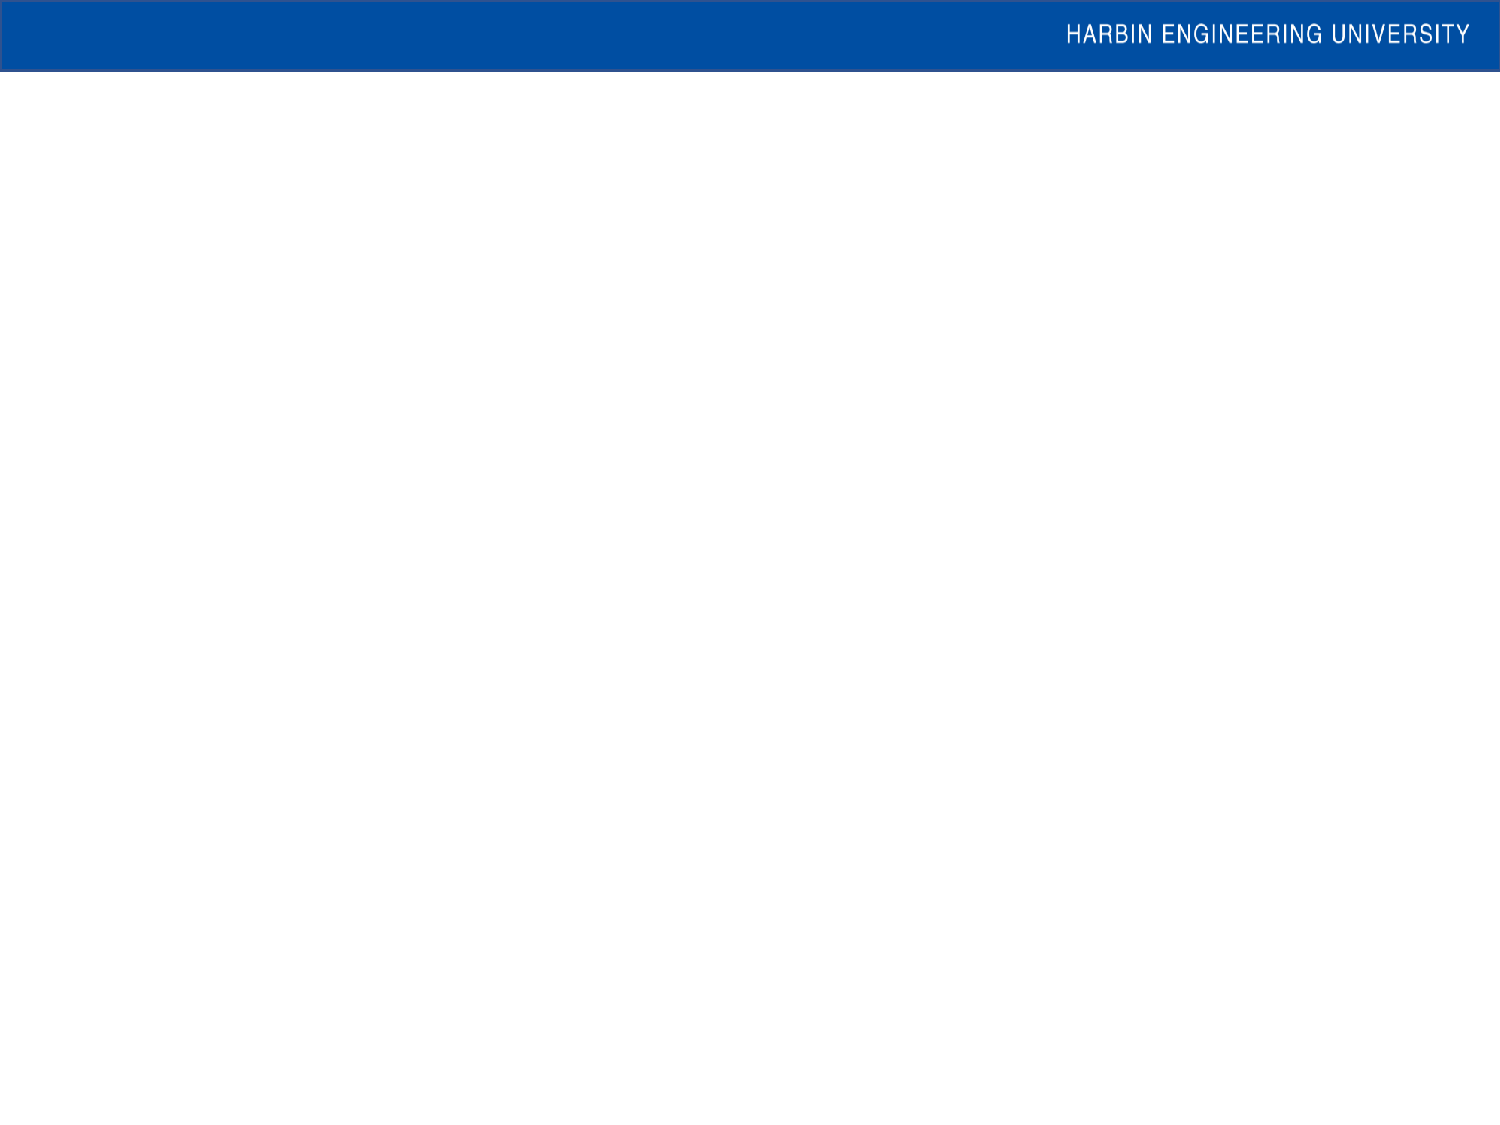
\includegraphics[width=\paperwidth,height=.98\paperheight]{./Themes/content4_3}
}
\usepackage[utf8]{inputenc}
\usepackage[english]{babel}
% Packages needed for algorithms and pseudocode
\usepackage{algorithm, algorithmic}
%\usepackage{algpseudocode}
%\usepackage[ruled,vlined]{algorithm2e}
% Package needed for mathematical symbols and formatting
\usepackage{amsmath}
\usepackage{ctex}
\usepackage{amsfonts}
\usepackage{amssymb}
\usepackage{ragged2e}
\usepackage{graphicx}
\graphicspath{{./Images}}
\author{Zefei Wu}
%\title{Chirst Univeristy Template}
%\subtitle{Subtitle here}
\setbeamercovered{transparent} 
% \institute[Assistant Professor]{Assistant Professor, \\ Department of Computer Science,\\ School of Sciences, \\ Christ (Deemed to be University),\\ Central Campus, Bengaluru} 
\date{} 
%\subject{} 
\addtobeamertemplate{frametitle}{\vspace*{0.3cm}}{\vspace*{0.2cm}}

\begin{document}
\setbeamertemplate{navigation symbols}{}

\title{ChatGPT Share}
\subtitle{}
{
\setbeamertemplate{background}{
\includegraphics[width=\paperwidth,height=.98\paperheight]{./Themes/main4_3.pdf}}
\begin{frame}
\vspace{.5cm}
\titlepage
\end{frame}
}

\begin{frame}{Table of Contents}
    \tableofcontents
\end{frame}

\section{ChatGPT介绍}
\begin{frame}{ChatGPT介绍}
\justifying
    \begin{figure}[htbp]
        \centering
        \begin{minipage}[b]{0.49\linewidth}
            \centering
            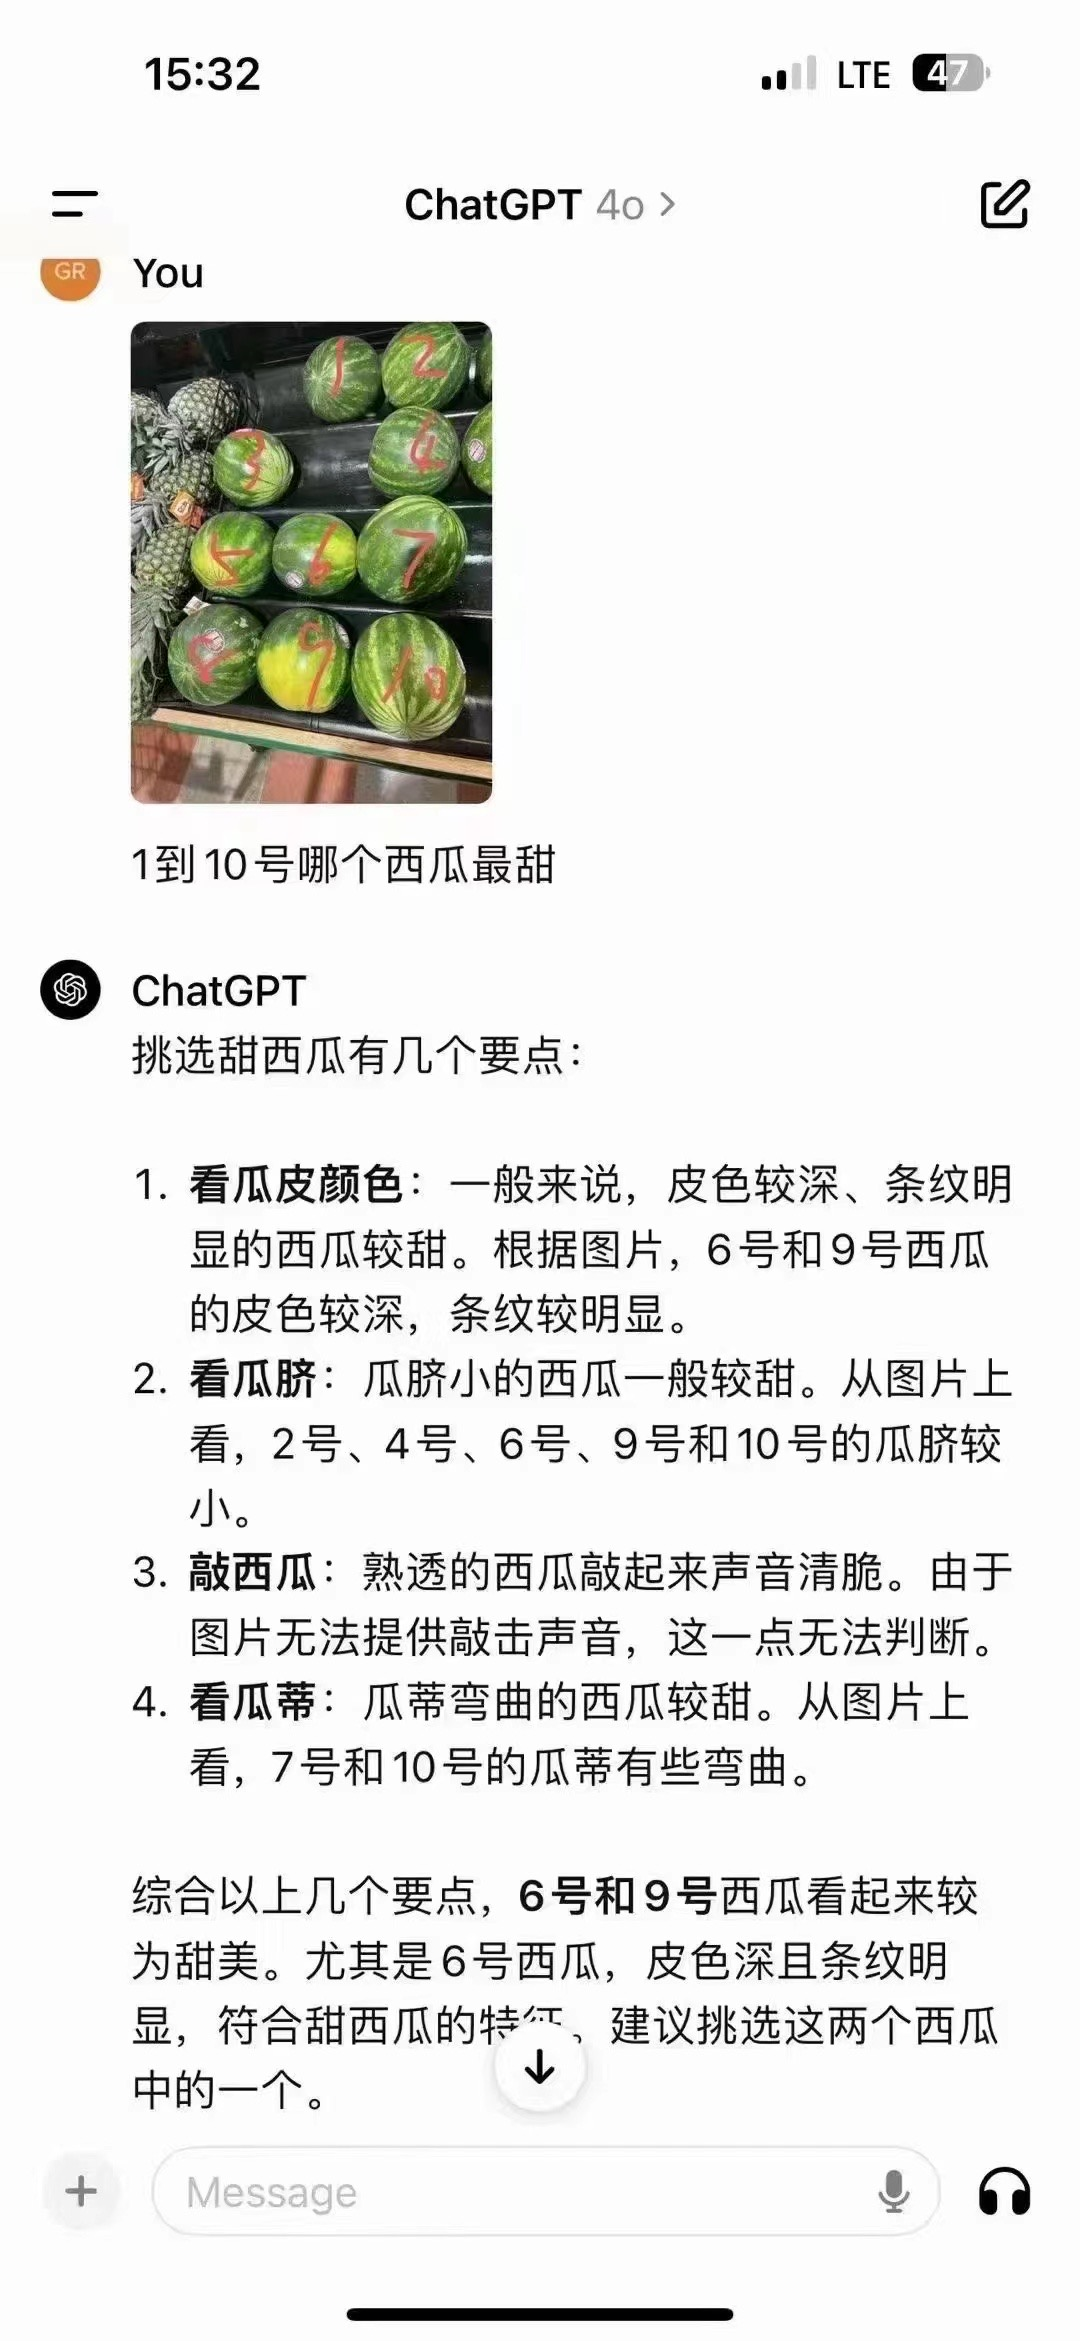
\includegraphics[height=0.6\textheight]{Images/1.jpg}
            \caption{咨询ChatGPT买西瓜}
            \label{fig:enter-label1}
        \end{minipage}
        \hfill
        \begin{minipage}[b]{0.49\linewidth}
            \centering
            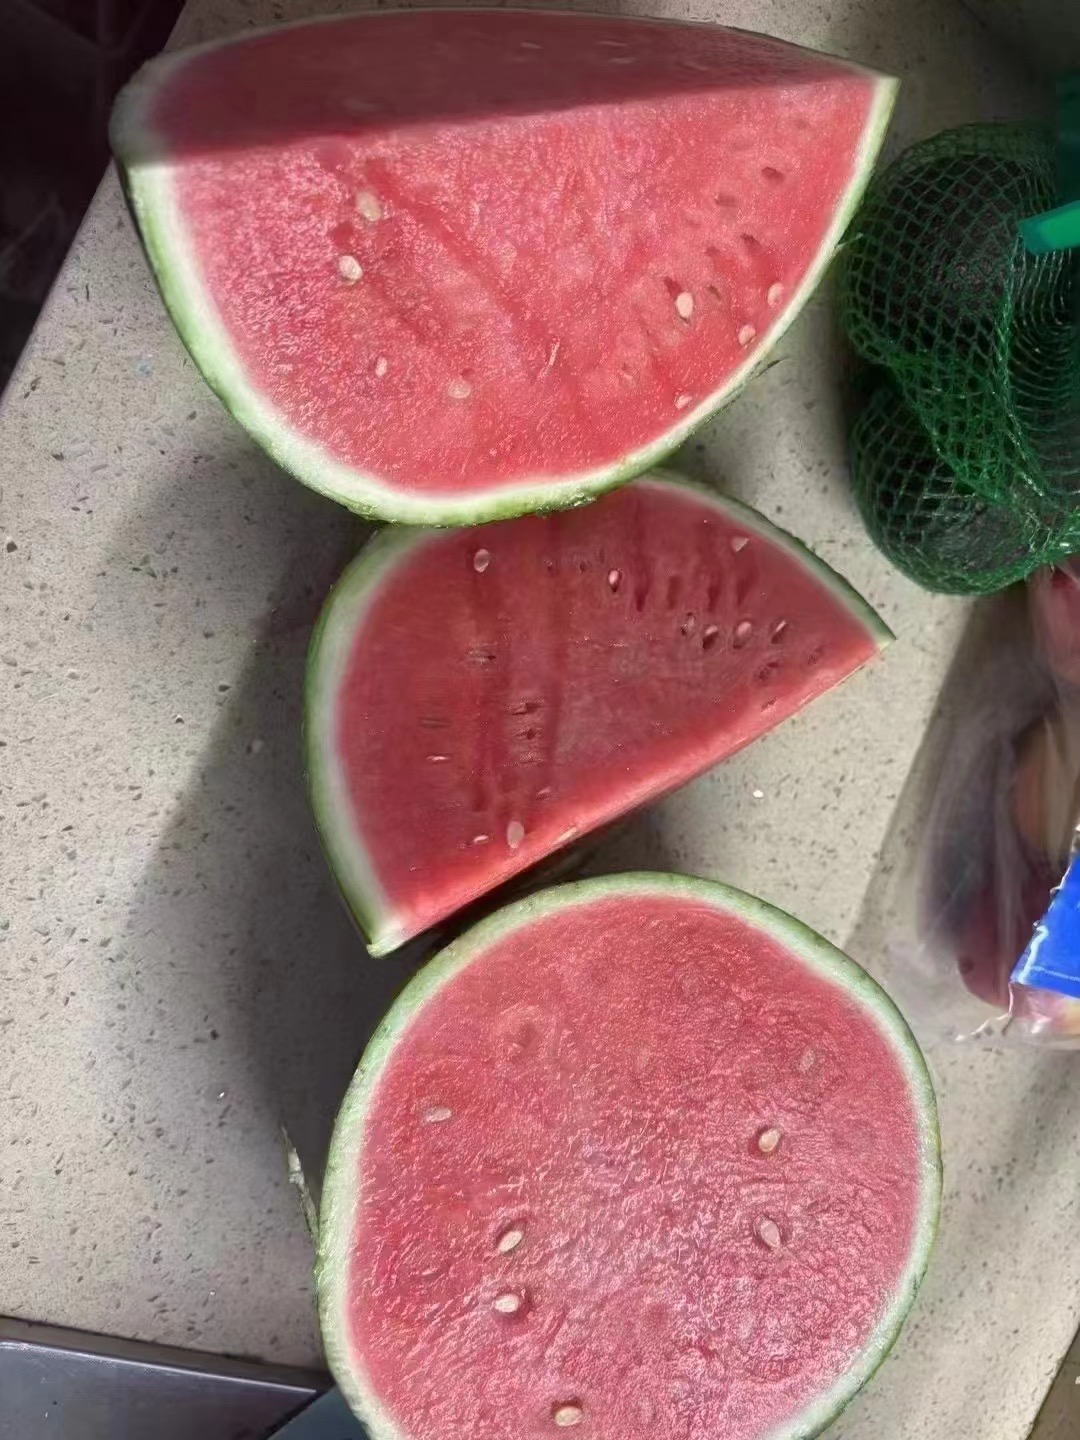
\includegraphics[height=0.6\textheight]{Images/2.jpg}
            \caption{真实买到的西瓜}
            \label{fig:enter-label2}
        \end{minipage}
    \end{figure}
\end{frame}

\section{注册 + VPN + 4Plus}
\begin{frame}{注册+VPN+4 Plus}
\justifying
    \begin{itemize}
        \item \href{https://www.youtube.com/watch?v=KzvBFQOXUaw&t=106s}{谷歌账号注册教程}
        \item \href{https://github.com/Z-Siqi/Clash-for-Windows_Chinese}{clash} + \href{https://fbweb02.flyingbird.la}{flyingbird} or \href{https://bbxy.info/user}{百变小樱}
        \item \hyperlink{item3}{升级ChatGPT4 plus}
            \\visa卡 or 礼品卡
    \end{itemize}
\end{frame}


\section{阅读文献}
\begin{frame}{阅读文献}
\centering
\justifying
    \begin{itemize}
        \item 研究目的和问题:明确该研究的核心关注点。
        \item 研究背景和理论基础:了解文献所依赖的背景信息和理论基础框架。
        \item 研究方法:详细了解文献中的研究设计、数据收集和分析方法。这有助于评估研究的可靠性和有效性。
        \item 研究结果:了解文献中呈现的主要研究结果和发现。
        \item 研究的局限性:识别研究中的不足和改进方向。
        \item 研究的创新性和贡献:是否提出了新的理论、方法或观点。
        \item 实际应用价值:评估它是否对实践有指导意义或能解决现实问题。
    \end{itemize}
\end{frame}


\section{学术润色}
\begin{frame}{学术润色}
\centering
\justifying
    \begin{itemize}

        \item \href{https://mp.weixin.qq.com/s/WzZS1tkxhylAbT6bSjKQGw}{50个ChatGPT学术指令}
        \item  \href{https://www.nature.com/articles/d41586-024-01042-3}{Three ways ChatGPT helps me in my academic writing}
    \end{itemize}
\end{frame}


\section{提示词}
\begin{frame}{提示词}
\centering
\justifying

    \begin{itemize}
        \item \href{https://github.com/f/awesome-chatgpt-prompts}{Awesome ChatGPT Prompts}
        \item \href{https://github.com/PlexPt/awesome-chatgpt-prompts-zh}{ChatGPT 中文调教指南}
    \end{itemize}
     可以说GPT本就是一个巨大的金库,提示词好比金库的钥匙
\end{frame}



\section{AI 内容检查工具}
\begin{frame}{AI 内容检查工具}
\centering
\justifying
    \begin{itemize}
        \item \href{https://app.gptzero.me/app/ai-scan?tab=0}{GPTZero}
        \item \href{https://originality.ai/}{Originality.ai}
        \item \href{https://www.turnitin.com/}{turnitin}
    \end{itemize}
    如果一个人会轻信GPTzero的结果,我觉得他不应该有掌握别人文章生死的权力,因为他的判断力和独立思考能力是匮乏的
    
    
\end{frame}


\end{document}
